%%%%%%%%%%%%%%%%%%%%%%%%%%%%% Define Article %%%%%%%%%%%%%%%%%%%%%%%%%%%%%%%%%%
\documentclass{article}
%%%%%%%%%%%%%%%%%%%%%%%%%%%%%%%%%%%%%%%%%%%%%%%%%%%%%%%%%%%%%%%%%%%%%%%%%%%%%%%

%%%%%%%%%%%%%%%%%%%%%%%%%%%%% Using Packages %%%%%%%%%%%%%%%%%%%%%%%%%%%%%%%%%%
\usepackage{geometry}
\usepackage{graphicx}
\usepackage{amssymb}
\usepackage{amsmath}
\usepackage{amsthm}
\usepackage{empheq}
\usepackage{mdframed}
\usepackage{booktabs}
\usepackage{lipsum}
\usepackage{graphicx}
\usepackage{color}
\usepackage{psfrag}
\usepackage{pgfplots}
\usepackage{bm}
\usepackage{indentfirst}
\usepackage{enumitem}
%%%%%%%%%%%%%%%%%%%%%%%%%%%%%%%%%%%%%%%%%%%%%%%%%%%%%%%%%%%%%%%%%%%%%%%%%%%%%%%

% Other Settings

%%%%%%%%%%%%%%%%%%%%%%%%%% Page Setting %%%%%%%%%%%%%%%%%%%%%%%%%%%%%%%%%%%%%%%
\geometry{a4paper}

%%%%%%%%%%%%%%%%%%%%%%%%%% Define some useful colors %%%%%%%%%%%%%%%%%%%%%%%%%%
\definecolor{ocre}{RGB}{243,102,25}
\definecolor{mygray}{RGB}{243,243,244}
\definecolor{deepGreen}{RGB}{26,111,0}
\definecolor{shallowGreen}{RGB}{235,255,255}
\definecolor{deepBlue}{RGB}{61,124,222}
\definecolor{shallowBlue}{RGB}{235,249,255}
%%%%%%%%%%%%%%%%%%%%%%%%%%%%%%%%%%%%%%%%%%%%%%%%%%%%%%%%%%%%%%%%%%%%%%%%%%%%%%%

%%%%%%%%%%%%%%%%%%%%%%%%%% Define an orangebox command %%%%%%%%%%%%%%%%%%%%%%%%
\newcommand\orangebox[1]{\fcolorbox{ocre}{mygray}{\hspace{1em}#1\hspace{1em}}}
%%%%%%%%%%%%%%%%%%%%%%%%%%%%%%%%%%%%%%%%%%%%%%%%%%%%%%%%%%%%%%%%%%%%%%%%%%%%%%%

%%%%%%%%%%%%%%%%%%%%%%%%%%%% English Environments %%%%%%%%%%%%%%%%%%%%%%%%%%%%%
\newtheoremstyle{mytheoremstyle}{3pt}{3pt}{\normalfont}{0cm}{\rmfamily\bfseries}{}{1em}{{\color{black}\thmname{#1}~\thmnumber{#2}}\thmnote{\,--\,#3}}
\newtheoremstyle{myproblemstyle}{3pt}{3pt}{\normalfont}{0cm}{\rmfamily\bfseries}{}{1em}{{\color{black}\thmname{#1}~\thmnumber{#2}}\thmnote{\,--\,#3}}
\theoremstyle{mytheoremstyle}
\newmdtheoremenv[linewidth=1pt,backgroundcolor=shallowGreen,linecolor=deepGreen,leftmargin=0pt,innerleftmargin=20pt,innerrightmargin=20pt,]{theorem}{Theorem}[section]
\theoremstyle{mytheoremstyle}
\newmdtheoremenv[linewidth=1pt,backgroundcolor=shallowBlue,linecolor=deepBlue,leftmargin=0pt,innerleftmargin=20pt,innerrightmargin=20pt,]{definition}{Definition}[section]
\theoremstyle{myproblemstyle}
\newmdtheoremenv[linecolor=black,leftmargin=0pt,innerleftmargin=10pt,innerrightmargin=10pt,]{problem}{Problem}[section]
%%%%%%%%%%%%%%%%%%%%%%%%%%%%%%%%%%%%%%%%%%%%%%%%%%%%%%%%%%%%%%%%%%%%%%%%%%%%%%%

%%%%%%%%%%%%%%%%%%%%%%%%%%%%%%% Plotting Settings %%%%%%%%%%%%%%%%%%%%%%%%%%%%%
\usepgfplotslibrary{colorbrewer}
\pgfplotsset{width=8cm,compat=1.9}
%%%%%%%%%%%%%%%%%%%%%%%%%%%%%%%%%%%%%%%%%%%%%%%%%%%%%%%%%%%%%%%%%%%%%%%%%%%%%%%

%%%%%%%%%%%%%%%%%%%%%%%%%%%%%%% Title & Author %%%%%%%%%%%%%%%%%%%%%%%%%%%%%%%%
\title{Homework 4}
\author{Nguyen Tuan Anh}
%%%%%%%%%%%%%%%%%%%%%%%%%%%%%%%%%%%%%%%%%%%%%%%%%%%%%%%%%%%%%%%%%%%%%%%%%%%%%%%

\begin{document}
    \maketitle
    \section*{Section 6.3}
    \subsection*{Exercise 39}
    How many bit strings of length 10 contain at least three
    1s and at least three 0s?
    \subsubsection*{Solution}
    In this problem, we will take the general case of bit strings length 10 and then minus
    for some specific cases that are not in the requirement of the problem.
    \begin{enumerate}
        \item There are 10 1s in the strings and 10 0s in the strings and there will be 
        one way for each so that in total there will be 2 ways
        \item There are 2 1s and 8 0s in the strings: $ ^2C_10 = \frac{10!}{2!\times(10 - 2)!} = 45 $ strings
        \item There are 1 1s and 9 0s in the strings: $ ^1C_10 = 10 $ strings
        \item There are 2 0s and 8 1s in the strings: $ ^2C_10 = \frac{10!}{2!\times(10 - 2)!} = 45 $ strings
        \item There are 1 0s and 9 1s in the strings: $ ^1C_10 = 10 $ strings
    \end{enumerate}
    $ \rightarrow $ The number of bit strings length 10 contain at least three 1s and at least three 0s:
    \begin{align*}
        2^{10} - (45 + 45 + 10 + 10) = 912 \ strings
    \end{align*}
    \subsection*{Exercise 40}
    How many ways are there to select 12 countries in the
    United Nations to serve on a council if 3 are selected from
    a block of 45, 4 are selected from a block of 57, and the
    others are selected from the remaining 69 countries?
    \subsubsection*{Solution}
    The ways are there to select 12 countries in the United Nations to serve on a council:
    \begin{align*}
        ^3C_{45} \times \ ^4C_{57} \times \ ^{(12 - 3 - 4)}C_{69} = 6.3 \times 10^{16} 
    \end{align*}
    \subsection*{Exercise 41}
    How many license plates consisting of three letters followed by three digits contain no letter or digit twice?
    \subsubsection*{Solution}
    As we know that there are 26 letters in the alphabet and 10 numbers in the integer.
    In this problem, we need to take 3 letters from 26 letters and matter the order, and we 
    also need to take 3 numbers from 10 numbers and matter the order. Therefore, we will use
    \textbf{Permutations}:\\
    
    For the letter, the way to choose 3 letters that are different from each other is : $ ^3P_{26} = 15600 $\\

    For the number, the way to choose 3 numbers that are different from each other is : $ ^3P_{10} = 720 $\\

    $ \rightarrow $ The number of license plates that satisfy with the requirement of the problem:
    \begin{align*}
        15600 \times 720 = 11,232,000 \ plates
    \end{align*}
    \subsection*{Exercise 43}
    Find a formula for the number of circular \(r\)-permutations of \(n\) people.
    \subsubsection*{Solution}
    We can see that for normal table, the \(r\) - permutations of \(n\) people will be \(^rP_n\) but in circular
    will be different because in the circular, there will be some cases that will be the same with each other if we rotate
    the circle. \\ 
    \begin{center}
        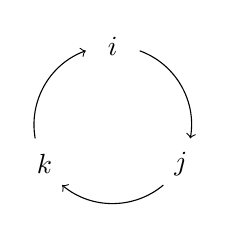
\begin{tikzpicture}[->,scale = 1]
            \node (i) at (90:1cm)  {$i$};
            \node (j) at (-30:1cm) {$j$};
            \node (k) at (210:1cm) {$k$};
        
            \draw (70:1cm)  arc (70:-10:1cm);
            \draw (-50:1cm) arc (-50:-130:1cm);
            \draw (190:1cm) arc (190:110:1cm);
        \end{tikzpicture}
        \space
        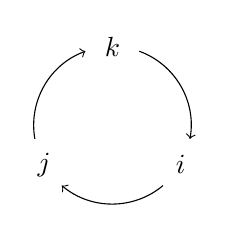
\begin{tikzpicture}[->,scale = 1]
            \node (i) at (90:1cm)  {$k$};
            \node (j) at (-30:1cm) {$i$};
            \node (k) at (210:1cm) {$j$};
        
            \draw (70:1cm)  arc (70:-10:1cm);
            \draw (-50:1cm) arc (-50:-130:1cm);
            \draw (190:1cm) arc (190:110:1cm);
        \end{tikzpicture}
        \space
        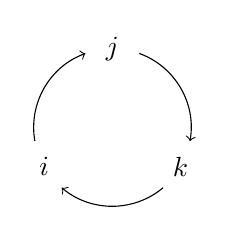
\begin{tikzpicture}[->,scale = 1]
            \node (i) at (90:1cm)  {$j$};
            \node (j) at (-30:1cm) {$k$};
            \node (k) at (210:1cm) {$i$};
        
            \draw (70:1cm)  arc (70:-10:1cm);
            \draw (-50:1cm) arc (-50:-130:1cm);
            \draw (190:1cm) arc (190:110:1cm);
        \end{tikzpicture}
    \end{center}
    For example, let take \(n = 3\) and we will need to find the 3 - permutations of 3 people. Basically, we will calculate by
    \(3! = 6\). However, on the picture above, we can see that there are 3 permutations but these permutations are the same
    because by rotating the circle, we will get second and the third from the first one. If we write all of the permutation as usual on
    the circular, it will be: \\ 
    \begin{center}
        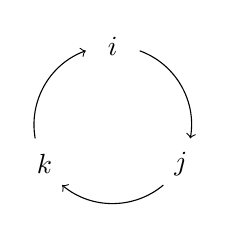
\begin{tikzpicture}[->,scale = 1]
            \node (i) at (90:1cm)  {$i$};
            \node (j) at (-30:1cm) {$j$};
            \node (k) at (210:1cm) {$k$};
        
            \draw (70:1cm)  arc (70:-10:1cm);
            \draw (-50:1cm) arc (-50:-130:1cm);
            \draw (190:1cm) arc (190:110:1cm);
        \end{tikzpicture}
        \space
        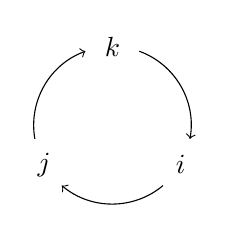
\begin{tikzpicture}[->,scale = 1]
            \node (i) at (90:1cm)  {$k$};
            \node (j) at (-30:1cm) {$i$};
            \node (k) at (210:1cm) {$j$};
        
            \draw (70:1cm)  arc (70:-10:1cm);
            \draw (-50:1cm) arc (-50:-130:1cm);
            \draw (190:1cm) arc (190:110:1cm);
        \end{tikzpicture}
        \space
        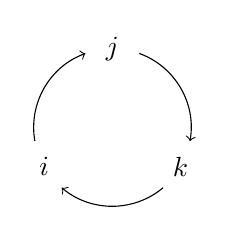
\begin{tikzpicture}[->,scale = 1]
            \node (i) at (90:1cm)  {$j$};
            \node (j) at (-30:1cm) {$k$};
            \node (k) at (210:1cm) {$i$};
        
            \draw (70:1cm)  arc (70:-10:1cm);
            \draw (-50:1cm) arc (-50:-130:1cm);
            \draw (190:1cm) arc (190:110:1cm);
        \end{tikzpicture}
        
        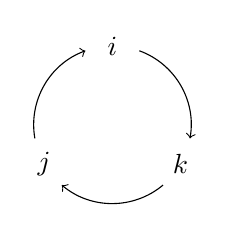
\begin{tikzpicture}[->,scale = 1]
            \node (i) at (90:1cm)  {$i$};
            \node (j) at (-30:1cm) {$k$};
            \node (k) at (210:1cm) {$j$};
        
            \draw (70:1cm)  arc (70:-10:1cm);
            \draw (-50:1cm) arc (-50:-130:1cm);
            \draw (190:1cm) arc (190:110:1cm);
        \end{tikzpicture}
        \space
        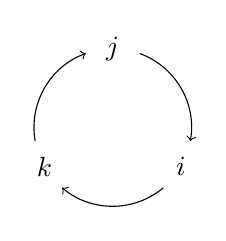
\begin{tikzpicture}[->,scale = 1]
            \node (i) at (90:1cm)  {$j$};
            \node (j) at (-30:1cm) {$i$};
            \node (k) at (210:1cm) {$k$};
        
            \draw (70:1cm)  arc (70:-10:1cm);
            \draw (-50:1cm) arc (-50:-130:1cm);
            \draw (190:1cm) arc (190:110:1cm);
        \end{tikzpicture}
        \space
        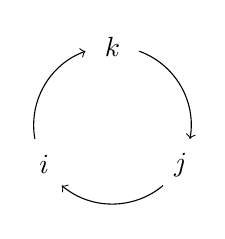
\begin{tikzpicture}[->,scale = 1]
            \node (i) at (90:1cm)  {$k$};
            \node (j) at (-30:1cm) {$j$};
            \node (k) at (210:1cm) {$i$};
        
            \draw (70:1cm)  arc (70:-10:1cm);
            \draw (-50:1cm) arc (-50:-130:1cm);
            \draw (190:1cm) arc (190:110:1cm);
        \end{tikzpicture}
    \end{center}
    Although on the picture show that there are 6 permutations but we just take first one on the first row and the
    second one on the second row. From that observation, we can give out the conclusion that for \(r\) people sitting on the
    table, we will have \(r\) way to rotate the table and we do not want to take the cases when we rotate the table so that
    we can get the formula:
    \begin{align*}
        P_3 = 3! = 6
    \end{align*}
    We do not want to take the rotation cases so that we will divide for the number of people sitting on the table. Because 
    there are 3 people so that we can get that:
    \begin{align*}
        \frac{P_3}{3} = \frac{3!}{3} = \frac{6}{3} = 2
    \end{align*}
    From this observation, we can get the formula when finding the \(n\) - permutations of \(n\) people:
    \begin{align*}
        \frac{P_n}{n} = \frac{n!}{n} = (n-1)!
    \end{align*}
    Moreover, if we are finding the number of circular \(r\)-permutations of \(n\) people. Firstly, we will choose \(r\) people
    from \(n\) people. And then, we will find the permutations of \(r\) people from the above formula. Choosing \(r\) people
    from \(n\) people, we will have that \(^rC_n\) and the permutations of \(r\) people will be \(\frac{r!}{r}\). Multiply them together,
    we will have that:
    \begin{align*}
        ^rC_n \times \frac{r!}{r} = \frac{n!}{r! \times (n - r)!} \times \frac{r!}{r} = \frac{n!}{r \times (n - r)!}
    \end{align*}
    \subsection*{Exercise 42}
    Find the number of circular 3-permutations of 5 people.
    \subsubsection*{Solution}
    Choose 3 from 5 people: \(^3C_5 = \frac{5!}{3! \times (5 - 3)!} = 10\)\\ 
    Permutations of 3 people: \((3 - 1)! = 2! = 2\)\\
    The number of circular 3 - permutations of 5 people: \(10 \times 2 = 20\)
    \subsection*{Exercise 44}
    Find a formula for the number of ways to seat \(r\) of \(n\) people around a circular table, where seatings are considered the same if every person has the same two neighbors without regard to which side these neighbors are sitting on.
    \subsubsection*{Solution}
    Let take the same example of \textbf{Exercise 43} where we find the circular 3 - permutations of 3 people, we will have that:
    \begin{center}
        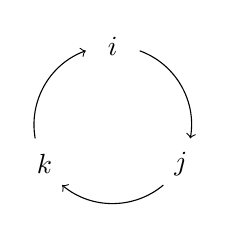
\begin{tikzpicture}[->,scale = 1]
            \node (i) at (90:1cm)  {$i$};
            \node (j) at (-30:1cm) {$j$};
            \node (k) at (210:1cm) {$k$};
        
            \draw (70:1cm)  arc (70:-10:1cm);
            \draw (-50:1cm) arc (-50:-130:1cm);
            \draw (190:1cm) arc (190:110:1cm);
        \end{tikzpicture}
        \space
        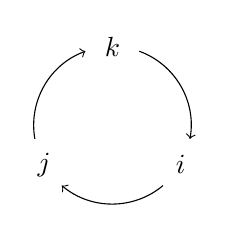
\begin{tikzpicture}[->,scale = 1]
            \node (i) at (90:1cm)  {$k$};
            \node (j) at (-30:1cm) {$i$};
            \node (k) at (210:1cm) {$j$};
        
            \draw (70:1cm)  arc (70:-10:1cm);
            \draw (-50:1cm) arc (-50:-130:1cm);
            \draw (190:1cm) arc (190:110:1cm);
        \end{tikzpicture}
        \space
        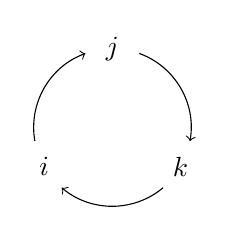
\begin{tikzpicture}[->,scale = 1]
            \node (i) at (90:1cm)  {$j$};
            \node (j) at (-30:1cm) {$k$};
            \node (k) at (210:1cm) {$i$};
        
            \draw (70:1cm)  arc (70:-10:1cm);
            \draw (-50:1cm) arc (-50:-130:1cm);
            \draw (190:1cm) arc (190:110:1cm);
        \end{tikzpicture}
        
        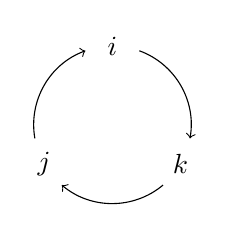
\begin{tikzpicture}[->,scale = 1]
            \node (i) at (90:1cm)  {$i$};
            \node (j) at (-30:1cm) {$k$};
            \node (k) at (210:1cm) {$j$};
        
            \draw (70:1cm)  arc (70:-10:1cm);
            \draw (-50:1cm) arc (-50:-130:1cm);
            \draw (190:1cm) arc (190:110:1cm);
        \end{tikzpicture}
        \space
        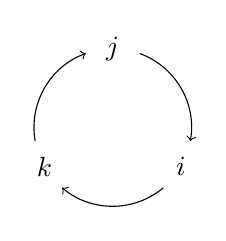
\begin{tikzpicture}[->,scale = 1]
            \node (i) at (90:1cm)  {$j$};
            \node (j) at (-30:1cm) {$i$};
            \node (k) at (210:1cm) {$k$};
        
            \draw (70:1cm)  arc (70:-10:1cm);
            \draw (-50:1cm) arc (-50:-130:1cm);
            \draw (190:1cm) arc (190:110:1cm);
        \end{tikzpicture}
        \space
        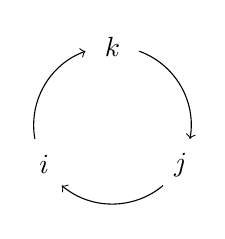
\begin{tikzpicture}[->,scale = 1]
            \node (i) at (90:1cm)  {$k$};
            \node (j) at (-30:1cm) {$j$};
            \node (k) at (210:1cm) {$i$};
        
            \draw (70:1cm)  arc (70:-10:1cm);
            \draw (-50:1cm) arc (-50:-130:1cm);
            \draw (190:1cm) arc (190:110:1cm);
        \end{tikzpicture}
    \end{center}
    In \textbf{Exercise 43}, the first row and the second row are two different permutations. However, on this
    problem requires that the first row and the second row are the same which means that they require the clockwise
    and anti-clockwise cases are all the same. Therefore, in this case, take the formula in \textbf{Exercise 43} and
    then divide by 2 because there are 2 direction clockwise and anti-clockwise and we commit that two of them
    are the same. We have the formula that:
    \begin{align*}
        \frac{P_n}{2 \times n} = \frac{n!}{2 \times n} = \frac{(n - 1)!}{2}
    \end{align*}
    Therefore, the circular \(r\) - permutations of \(n\) people we will first choose \(r\) people from \(n\) people and then
    use the circular \(r\)-permutations of \(n\) people:
    \begin{align*}
        ^rC_k \times \frac{P_n}{2 \times n} = \frac{n!}{r! \times (n - r)!} \times \frac{r!}{2 \times r} = \frac{n!}{2 \times r \times (n -r)!}
    \end{align*}
    \section*{Section 6.4}
    \subsection*{Exercise 21}
    Show that if \(n\) and \(k\) are integers with \(1 \leq k \leq n\), then \(\binom{n}{k} \leq \frac{n^k}{2^{k - 1}}\)
    \subsection*{Solution}
    \begin{itemize}
        \item For \(k = 1\), the inequation will become:
        \begin{align*}
            \frac{n!}{1! \times (n - 1)!} = \frac{n}{2^{1 - 1}} \leftrightarrow n = n
        \end{align*}
        Therefore, we will have the case when \(k = 1\) the inequation will be equal.
        \item For \(k = 2\), the inequation will become:
        \begin{align*}
            \frac{n!}{2! \times (n - 2)!} &< \frac{n^2}{2^{2 - 1}}\\
            \leftrightarrow \frac{n \times (n - 1)}{2} &< \frac{n \times n}{2}
        \end{align*}
        \item For \(k = n - 1\), the inequation will become:
        \begin{align*}
            \frac{n!}{(n - 1)! \times (n - n + 1)!} &< \frac{n^{n - 1}}{2^{n - 1 - 1}}\\
            \leftrightarrow n &< \frac{n^{n - 1}}{2^{n - 2}}
        \end{align*}
        \item For \(k = n\), the inequation will become:
        \begin{align*}
            \frac{n!}{n! \times (n - n) !} &< \frac{n^n}{2^{n - 1}}\\ 
            \leftrightarrow 1 &< \frac{n^n}{2^{n - 1}}
        \end{align*}
    \end{itemize}
    Because the cases \(k = n - 1\) and \(k = n\) are all \textbf{true} value for any \(n\), when \(k \neq 1\) the inequation
    will not have the equal operator. And when \(k = 1\), it will make the inequation become equal to each other. Therefore, we can prove that:
    \begin{align*}
        \binom{n}{k} \leq \frac{n^k}{2^{k - 1}}
    \end{align*}
    \subsection*{Exercise 22}
    Suppose that b is an integer with \(b \leq 7\). Use the binomial theorem and the appropriate row of Pascal’s triangle
    to find the base-b expansion of \((11)^4_b\).
    \subsubsection*{Solution}
    Firstly, we will need to convert \(11_b\) into decimal: \(11_b = 1 \times b^1 + 1 \times b^ 0 = b + 1\). Secondly, we will have
    the the fourth power of \((b + 1)\): \((b + 1)^4 = b^4 + 4b^3 + 6b^2 + 4b + 1\). Because we have that \(b \geq 7\) so that the number in base \(b\)
    will start from \{0,1,2,3,4,5,6,..., \(b-1\)\}. Therefore, the binomial coefficients will be a single digit because the largest coefficients in the
    equation is 6 and it can be respresented if and only the base \(b \geq 7\). So the number will be:
    \begin{align*}
        1 \times b^4 + 4 \times b^3 + 6 \times b^2 + 4 \times b + 1 \times b^0
    \end{align*} 
    Take all the number stand before \(b\), we will have that \((14641)_b\)
    \subsection*{Exercise 23}
    Prove Pascal’s identity, using the formula for \(\binom{n}{r}\)
    \subsubsection*{Solution}
    We have that:
    \begin{align*}
        \binom{n}{k - 1} + \binom{n}{k} &= \frac{n!}{(k - 1)! \times (n - k + 1)!} + \frac{n!}{k! \times (n - k)!}\\ 
        &= \frac{n! \times k}{k! \times (n - k + 1)!} + \frac{n! \times (n - k + 1)}{k! \times (n - k + 1)!}\\ 
        &= \frac{n! \times (k + n - k + 1)}{k! \times (n - k + 1)!}\\ 
        &= \frac{n! \times (n + 1)}{k! \times (n - k + 1)!} \\
        &= \frac{(n + 1)!}{k! \times (n + 1 - k)!} = \binom{n + 1}{k}
    \end{align*}
    \subsection*{Exercise 24}
    Suppose that k and n are integers with \(1 \leq k < n\). Prove the \textbf{hexagon identity}
    \begin{align*}
        \binom{n - 1}{k - 1}\binom{n}{k+1}\binom{n+1}{k} = \binom{n - 1}{k}\binom{n}{k - 1}\binom{n + 1}{k + 1}
    \end{align*}
    which relates terms in Pascal's triangle that form a hexagon.
    \subsubsection*{Solution}
    \begin{align*}
        \binom{n - 1}{k - 1}\binom{n}{k+1}\binom{n+1}{k} &= \binom{n - 1}{k}\binom{n}{k - 1}\binom{n + 1}{k + 1}\\
        \frac{(n - 1)!}{(k - 1)!(n - 1 - k + 1)!}\cdot\frac{n!}{(k + 1)!(n - k - 1)!}\cdot\frac{(n+1)!}{k!(n + 1 - k)!} &= \frac{(n - 1)!}{k!(n - 1 - k)!}\cdot\frac{n!}{(k - 1)!(n - k + 1)!}\\ &\cdot\frac{(n+1)!}{(k + 1)!(n + 1 - k - 1)!}\\
        \frac{(n - 1)! n! (n+1)!}{(k -1)!k!(k+1)!(n - k - 1)!(n - k)!(n - k + 1)!} &= \frac{(n - 1)!n!(n+1)!}{(k - 1)!k!(k+1)!(n-k-1)!(n-k)!(n-k+1)!}
    \end{align*}
    \subsection*{Exercise 25}
    Prove that if n and k are integers with \(1 \leq k \leq n\), then \(k\binom{n}{k} = n\binom{n - 1}{k - 1}\)
    \begin{enumerate} [label = (\alph*)]
        \item using a combinatorial proof.
        \item using an algebraic proof based on formula for \(\binom{n}{r}\) given in Theorem 2 in Section 6.3.
    \end{enumerate}
    \subsubsection*{Solution}
    \begin{enumerate} [label = (\alph*)]
        \item Consider that there is a class with \(n\) students with testscore \(\geq 80\) and we will pick \(k\) students to have a small special test in the class. And now, the teacher wants to choose one student from \(k\) students to participate in a
        contest.We will take this example to prove that \(k\binom{n}{k} = n\binom{n - 1}{k - 1}\).
        \begin{itemize}
            \item On the left hand side: So first we will pick \(k\) students from \(n\) students so we will have
            \(\binom{n}{k}\) ways. And then, we will have \(k\) way to choose a student who will participate in a contest.
            Therefore, we have that \(k \times \binom{n}{k}\) ways.
            \item On the right hand side: We know that the teacher will choose one student to participate in the contest so we can also choose
            the student who will participate in the contest first, Therefore, we will have \(n\) ways to choose that student. And now we will find
            the other students in \(k\) students. Because the student who participate in the contest are in the group \(k\) student so that we will choose \(k - 1\) students
            from \(n - 1\) students which means that \(\binom{n - 1}{k - 1}\). Therefore, we have that \(n \times \binom{n - 1}{k - 1}\).
        \end{itemize}
        We can see that, the left hand side and the right hand side option although has different formulas, the result they give all the same
        because the final result is choosing the student who participate in the contest and we all choose that students from a group of \(k\) students from the class has \(n\) students.
        \item We have that:
        \begin{align*}
            k\binom{n}{k} &= k \times \frac{n!}{k!(n - k)!} = \frac{n!}{(k - 1)!(n - k)!}\\
            n\binom{n - 1}{k - 1} &= n \times \frac{(n - 1)!}{(k - 1)!(n - 1 - k + 1)!}  = \frac{n!}{(k - 1)!(n - k)!}
        \end{align*}
        Therefore, we can prove that \(k\binom{n}{k} = n\binom{n - 1}{k - 1}\)
    \end{enumerate}
    \subsection*{Exercise 26}
    Prove the identity \(\binom{n}{r}\binom{r}{k} = \binom{n}{k}\binom{n - k}{r - k}\), whenever \(n, r\) and
    \(k\) are nonnegative integers with \(r \leq n\) and \(k \leq r\),
    \begin{enumerate} [label = (\alph*)]
        \item using a combinatorial argument
        \item using an argument based on the formula for the number of \(r\)-combinations of a set with \(n\) elements.
    \end{enumerate}
\end{document}